\documentclass[12pt]{article}
\usepackage[hmargin=1.8cm,vmargin=1.4cm,includehead,includefoot]{geometry}
\usepackage{graphicx}
\usepackage{pdfpages}
\usepackage{fancyhdr}


\begin{document}

\setcounter{page}{0}
\thispagestyle{empty}

\vspace*{2cm}

\begin{center}
\Huge{\sffamily Institute for Mathematical Informatics}\\
\vspace{1.5cm}
\Huge{\sffamily Annual Report}\\
\vspace{0.5cm}
\Huge{\sffamily 2024}

\vfill

\includegraphics[scale=0.75]{circle_logo.pdf}
\vfill

\Huge{M}\Large{EIJI}
\Huge{G}\Large{AKUIN}
\Huge{U}\Large{NIVERSITY}
\end{center}

\vspace{1cm}

\newpage

\pagestyle{fancy}
\fancyhead{}
\fancyhead[L]{\usefont{OT1}{phv}{m}{n}MGU-IMI Annual Report}
\fancyhead[R]{\usefont{OT1}{phv}{m}{n}Vol.~1 (2024)}
\fancyfoot{}
\fancyfoot[L]{\TheAuthor}
\fancyfoot[R]{\footnotesize \thepage}
\renewcommand{\footrulewidth}{1pt}
\renewcommand{\headrulewidth}{1pt}

%
% Hideki Yukawa's contribution
%
\fancyfoot[L]{Hideki Yuakwa}
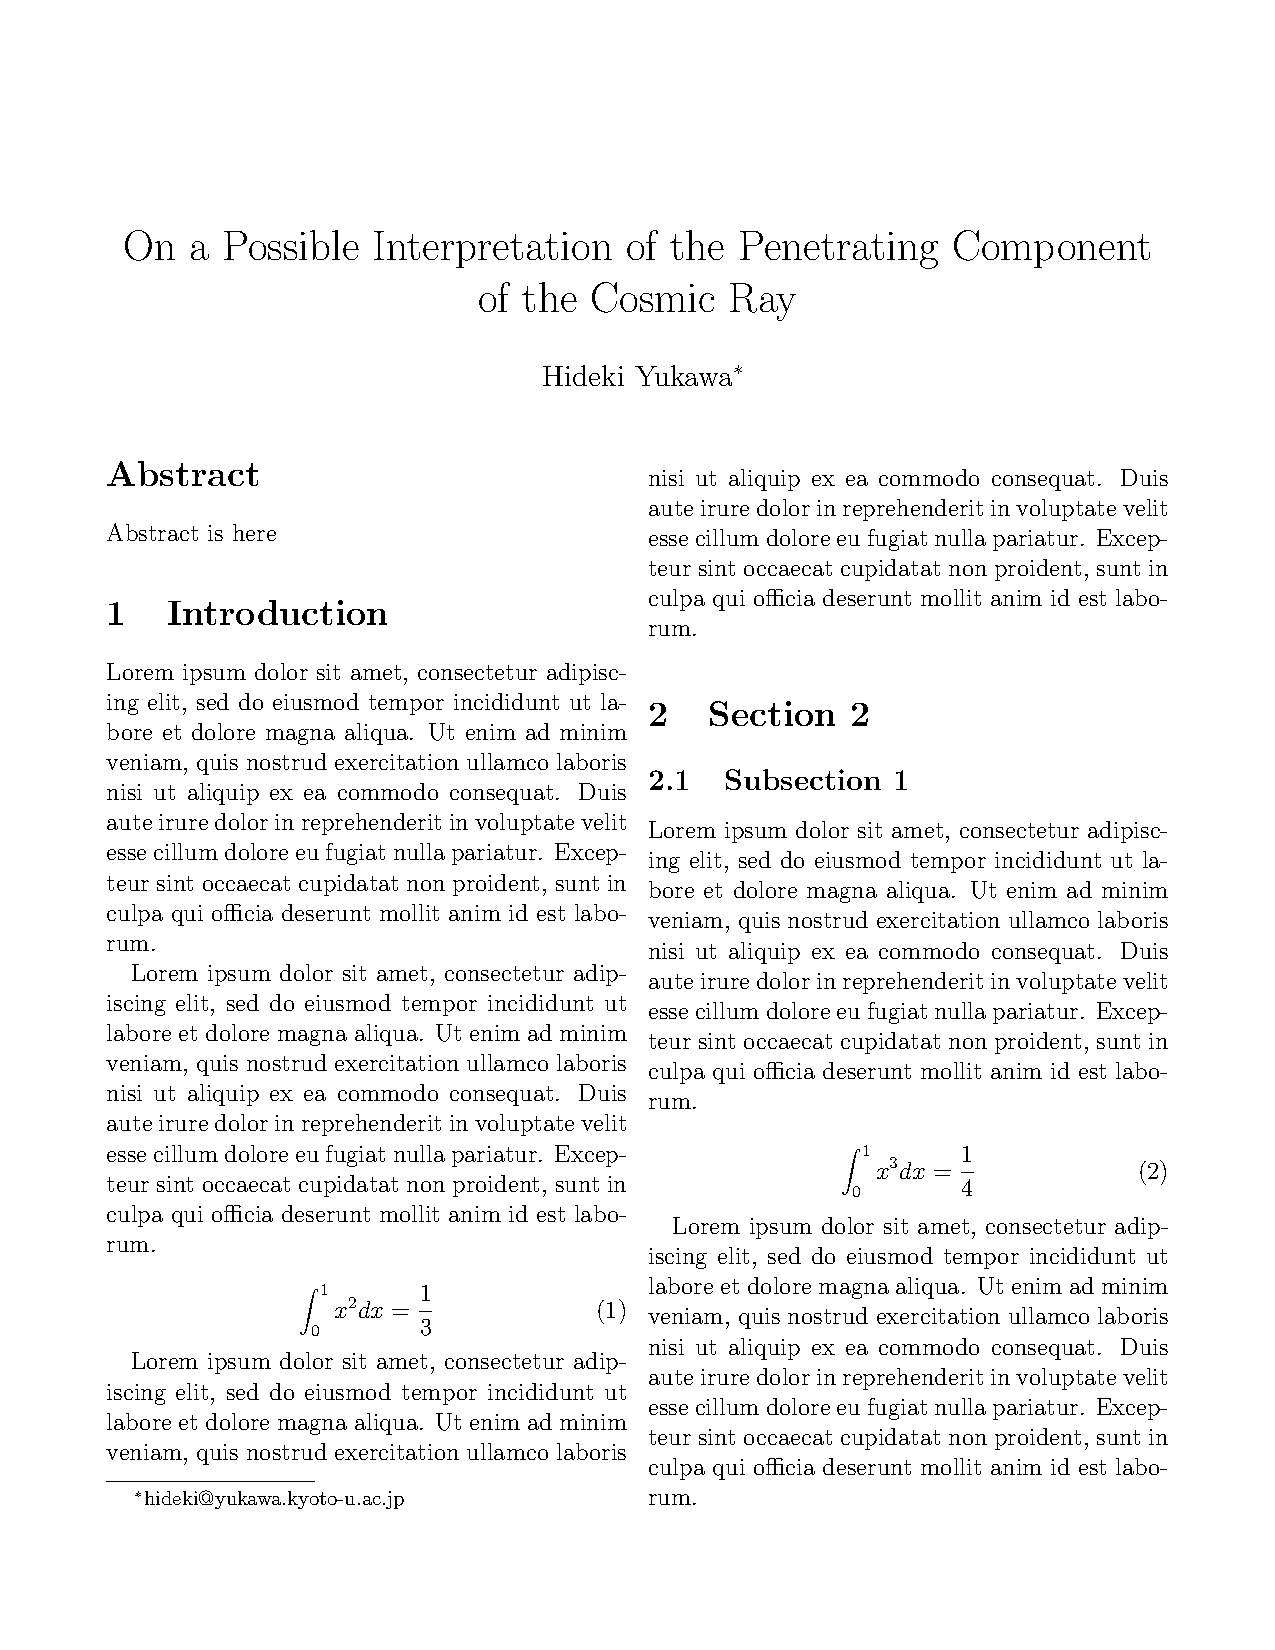
\includepdf[pages=-,pagecommand={\thispagestyle{fancy}}]{contribution1.pdf}

%
% Paul Dirac's contribution
%
\fancyfoot[L]{Paul Dirac}
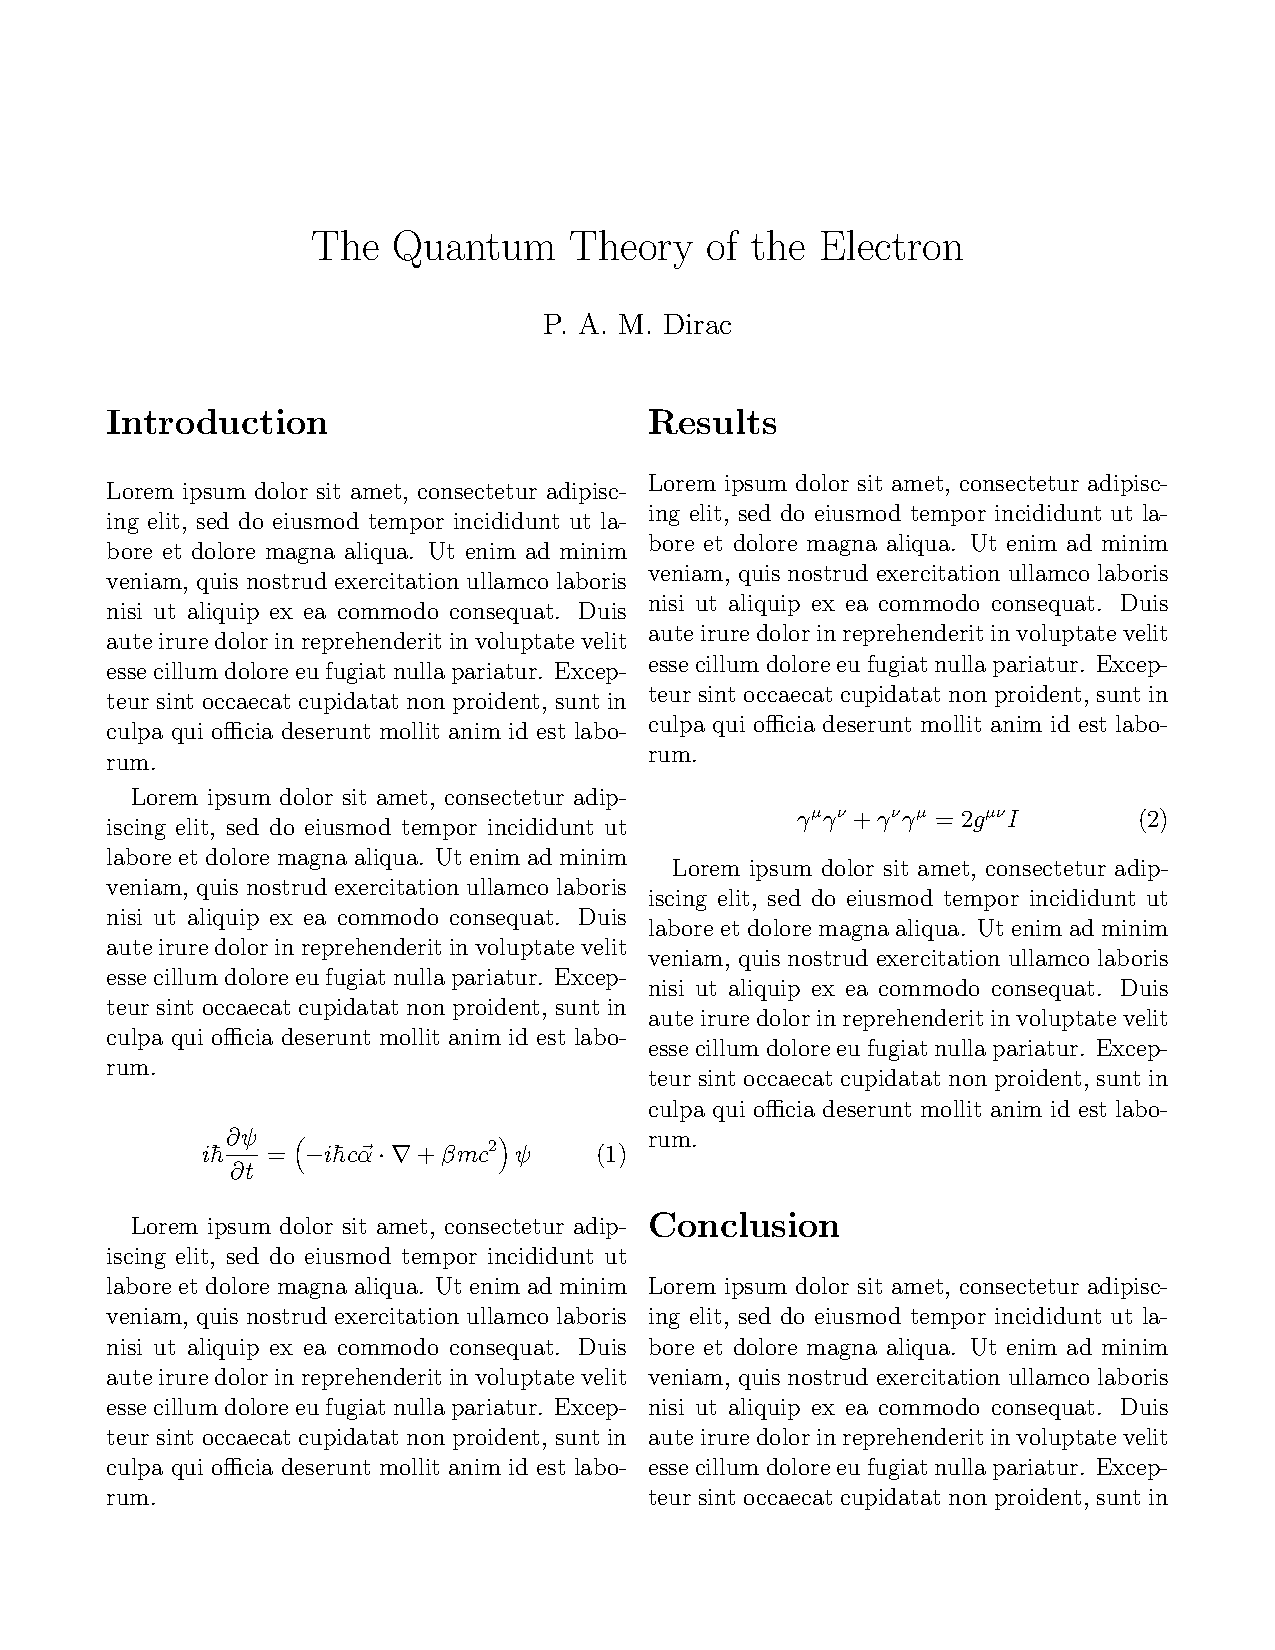
\includepdf[pages=-,pagecommand={\thispagestyle{fancy}}]{contribution2.pdf}

%
% Japanese LaTeX
%
\fancyfoot[L]{GitHub Copilot}

\includepdf[pages=-,pagecommand={\thispagestyle{fancy}}]{japanese.pdf}
 
\end{document}